\chapter{Implementation}

\section{Overview}

This chapter explains how the system was built. It covers the development environment, the
dataset preparation, the training pipeline, the text processing strategy, how class imbalance was
handled, the inference and ambiguity detection logic, and how the model is saved and loaded.

\section{Development Environment}

The system is implemented in Python 3.10. The main libraries used are:

\begin{itemize}
    \item \texttt{sentence-transformers}~\cite{sentence_bert}: For computing semantic embeddings using
    \texttt{all-mpnet-base-v2}.
    \item \texttt{scikit-learn}: For TF-IDF vectorization, nearest-neighbour indexing, and
    evaluation metrics.
    \item \texttt{xgboost}: For the classification models~\cite{xgboost_emotion}.
    \item \texttt{giotto-tda}~\cite{giotto}: For Vietoris-Rips persistence computation and Persistence
    Landscapes.
    \item \texttt{joblib}: For saving and loading the trained model to and from disk.
    \item \texttt{datasets}: For loading the GoEmotions dataset from the HuggingFace hub.
    \item \texttt{numpy} and \texttt{pandas}: For data manipulation.
    \item \texttt{torch}: For GPU-accelerated embedding computation during training.
    \item \texttt{teaspoon}~\cite{teaspoon}: For additional topological signal processing utilities.
\end{itemize}

During training, a GPU (CUDA-enabled) was used to speed up the embedding computation step.
The rest of the pipeline (TDA computation, XGBoost training) runs on CPU. Inference runs
entirely on CPU.

The code is organized into two main files: \texttt{tdanew4.py} for training and evaluation, and
\texttt{ambiguity.py} for interactive inference.

\section{Dataset Preparation}

The GoEmotions dataset (simplified version) is used~\cite{goemotions}. It was loaded from the HuggingFace
\texttt{datasets} library and cached locally so that training can proceed without an internet
connection after the first download. The annotation methodologies used in this dataset have
been subject to experimental analysis in recent literature~\cite{emotion_annotation}.

The dataset has 43,410 training samples and 5,427 test samples. Each sample is a Reddit
comment with one or more labels from 28 emotion categories.

The 28 emotion categories are mapped to three classes as shown in \textbf{Table~\ref{tab:label_map}}.

\begin{table}[H]
\centering
\caption{GoEmotions Label Mapping to Three Classes}
\label{tab:label_map}
\begin{tabular}{llp{5cm}}
\toprule
\textbf{Target Class} & \textbf{GoEmotions Indices} & \textbf{Example Emotions} \\
\midrule
Positive & 0, 1, 4, 5, 13, 15, 18, 20, 21, 24 & admiration, joy, pride, gratitude \\
Negative & 2, 3, 6, 7, 9, 10, 11, 12, 14, 16, 19, 22, 23, 25, 26 & anger, disgust, fear, sadness \\
Neutral  & 27 & neutral \\
\bottomrule
\end{tabular}
\end{table}

As shown in \textbf{Table~\ref{tab:label_map}}, the original GoEmotions labels are mapped to three
broad categories to simplify the classification task while preserving emotional valence.

Each sample can belong to more than one class because the original GoEmotions labels are
multi-label. A comment labelled as both ``joy'' and ``admiration'' would be mapped to Positive.
The labels are converted to a binary vector of length 3, where each position indicates membership
in that class.

\section{Text Processing Strategy}

In traditional natural language processing systems, text preprocessing steps such as
tokenization, stopword removal, stemming, and lemmatization are commonly applied before any
model training. These steps were designed for older models that worked on raw word counts and
needed clean, normalized input.

However, in this project, heavy text preprocessing was deliberately not applied. The reason
is that modern embedding models like \texttt{all-mpnet-base-v2} are trained on very large
datasets and can handle raw text directly. They have already learned to deal with capitalization,
punctuation, and common variations in word form. Applying aggressive preprocessing on top of
this would remove contextual information that the embedding model would otherwise use.

For example, removing stopwords from the sentence ``I am not happy at all'' would leave
``happy'', which could easily be misclassified as Positive. The full sentence, passed directly
to the embedding model, encodes the negation correctly.

More importantly, this project uses Topological Data Analysis on the geometric structure of the
embeddings. The topology depends on the exact positions of the vectors in the high-dimensional
space. If preprocessing changes the text before embedding, the geometry changes too, and the
topological features become less informative.

Therefore, raw text was passed directly to the embedding model with no preprocessing.
This preserves the full semantic richness of the input and maintains the meaningful geometric
structure that the topological analysis depends on.

The only preprocessing that was applied was the standard stopword removal inside the TF-IDF
vectorizer, which is appropriate because TF-IDF is a count-based model where common function
words genuinely do not add information.

\textbf{Table~\ref{tab:text_proc}} shows the comparison between traditional NLP preprocessing and the
approach used in this project.

\begin{table}[H]
\centering
\caption{Text Processing Strategy Comparison}
\label{tab:text_proc}
\begin{tabular}{ll}
\toprule
\textbf{Traditional NLP} & \textbf{This Project} \\
\midrule
Tokenization (manual) & Handled internally by embedding model \\
Stopword removal & Avoided for embeddings; used only in TF-IDF \\
Stemming / Lemmatization & Not applied \\
Manual feature engineering & Avoided \\
Dense embeddings & Used as primary representation \\
\bottomrule
\end{tabular}
\end{table}

As shown in \textbf{Table~\ref{tab:text_proc}}, the design choice to avoid traditional preprocessing
ensures that the semantic richness and geometric structure of the embeddings are preserved for
topological analysis.

This design choice ensures that the natural structure of language is preserved, which is important
for capturing semantic ambiguity through topology.

\section{Handling Class Imbalance}

The GoEmotions dataset has a significant class imbalance. After mapping, the Neutral class has
around 3,588 samples in the test set, while Positive has 1,189 and Negative has only 650. This
means that a naive classifier would be heavily biased toward Neutral.

SMOTE (Synthetic Minority Oversampling Technique) was considered as a solution but was
deliberately rejected. SMOTE works by creating interpolated synthetic data points between
existing minority class examples. This changes the embedding space by adding points that do
not correspond to real sentences. Since the topological analysis in this project depends on the
real geometry of the training embeddings, adding synthetic points would corrupt the topology
and make the ambiguity signal unreliable.

Instead, class imbalance was addressed through threshold tuning. Each of the three XGBoost
classifiers is a binary one-vs-rest model. By default, a probability of 0.5 or higher triggers a
positive prediction. In this project, the decision thresholds for each class were adjusted based
on the class distribution. Classes with fewer samples got lower thresholds, making the classifier
more sensitive to them.

This approach handles imbalance without modifying the underlying data or its geometric
structure. The topological analysis sees the real training distribution, which is exactly what we
want.

\section{Training Pipeline}

The training is performed in \texttt{tdanew4.py}. The steps are:

\begin{algorithm}[H]
\caption{Training Pipeline}
\label{alg:train}
\begin{algorithmic}[1]
\Require GoEmotions training split (43,410 samples)
\Ensure Saved model file \texttt{final\_model.joblib}
\State Load GoEmotions dataset (simplified version)
\State Map 28-class labels to 3-class binary vectors
\State Encode all training texts using \texttt{all-mpnet-base-v2} to get $X_{\text{dense}}$ (768-dim)
\State Encode all test texts using the same model
\State Fit TF-IDF vectorizer on training texts; transform train and test to get $X_{\text{tfidf}}$
\State Build nearest-neighbour index on $X^{\text{train}}_{\text{dense}}$ using cosine distance
\For{each sample $i$ in training set}
    \State Find 24 nearest neighbours of sample $i$ in $X^{\text{train}}_{\text{dense}}$
    \State Form point cloud from the 24 neighbour vectors (shape $1 \times 24 \times 768$)
    \State Compute Vietoris-Rips persistence diagram (H0 and H1)
    \State Extract Persistence Landscape (2 layers, 30 bins)
    \State Store flattened landscape as topological feature vector
\EndFor
\State Stack topological features as $X_{\text{topo}}$
\State Concatenate: $X_{\text{final}} = [X_{\text{dense}} \mid X_{\text{tfidf}} \mid X_{\text{topo}}]$
\State Repeat topology computation for test set using training neighbours
\For{each class $c \in \{\text{Positive, Negative, Neutral}\}$}
    \State Train XGBoost binary classifier on $X^{\text{train}}_{\text{final}}$, labels $y_c$
\EndFor
\State Evaluate on test set; compute accuracy, precision, recall, F1
\State Save all model components to \texttt{final\_model.joblib}
\end{algorithmic}
\end{algorithm}

The topology computation step is the most expensive. It is run in parallel using all available
CPU cores to reduce total training time. The full training run on 43,410 samples takes
approximately three to four hours on a CPU, or about 30 to 45 minutes with GPU-accelerated
embedding encoding.

\section{Inference and Ambiguity Detection}

The inference is handled in \texttt{ambiguity.py}. At startup, the saved model is loaded from
disk. The user enters text through the terminal, and the system processes it and returns a result.

\begin{algorithm}[H]
\caption{Inference and Ambiguity Detection}
\label{alg:infer}
\begin{algorithmic}[1]
\Require Input text $t$, saved model components
\Ensure Emotion label $\in \{\text{Positive, Negative, Neutral, Ambiguous}\}$
\State Encode $t$ using \texttt{all-mpnet-base-v2} to get $v_{\text{dense}}$
\State Extract TF-IDF features for $t$ using saved vectorizer to get $v_{\text{tfidf}}$
\State Retrieve 24 nearest neighbours of $v_{\text{dense}}$ from saved training embeddings
\State Compute Vietoris-Rips persistence on the 24-point neighbourhood
\State Extract Persistence Landscape to get $v_{\text{topo}}$
\State Concatenate: $v_{\text{final}} = [v_{\text{dense}} \mid v_{\text{tfidf}} \mid v_{\text{topo}}]$
\State Obtain probabilities: $p_{\text{pos}}, p_{\text{neg}}, p_{\text{neu}}$ from the three classifiers
\State Compute confidence gap: $\text{gap} = p_{\text{top1}} - p_{\text{top2}}$
\State Count H1 loops: $\text{loops} =$ number of H1 features in persistence diagram
\If{$\text{loops} \geq 14$}
    \State \Return \textsc{ambiguous} (extreme geometry)
\ElsIf{$\text{loops} \geq 10$ \textbf{and} $\text{gap} < 0.30$}
    \State \Return \textsc{ambiguous} (moderate geometry + low confidence)
\ElsIf{$\text{gap} < 0.10$}
    \State \Return \textsc{ambiguous} (very low confidence)
\Else
    \State \Return class with highest probability
\EndIf
\end{algorithmic}
\end{algorithm}

The system also prints debug information so the user can see what drove the decision. An
example of the debug output is:

\begin{verbatim}
--- DEBUG INFO ---
Input : i dont know how i feel
Probabilities : POS=0.0991 NEG=0.5271 NEU=0.3794
Confidence gap : 0.1477 (threshold < 0.30)
Loop count (H1): 15 (extreme >= 14, moderate >= 10)
Trigger : EXTREME topology
Final Result : AMBIGUOUS
\end{verbatim}

\section{Example Outputs}

\textbf{Table~\ref{tab:ex_outputs}} shows how the system responds to different types of inputs and which
rule was triggered.

\begin{table}[H]
\centering
\caption{Example System Inputs and Outputs}
\label{tab:ex_outputs}
\begin{tabular}{lccl}
\toprule
\textbf{Input} & \textbf{Loop Count} & \textbf{Confidence Gap} & \textbf{Result} \\
\midrule
I am very happy              & 4  & 0.40 & \textsc{positive} \\
I am sad                     & 11 & 0.86 & \textsc{negative} \\
shut up                      & 4  & 0.56 & \textsc{negative} \\
do this                      & 10 & 0.28 & \textsc{ambiguous} \\
i am fine                    & 3  & 0.35 & \textsc{positive} \\
i will kill you              & 4  & 0.06 & \textsc{ambiguous} \\
i dont know how i feel       & 15 & 0.15 & \textsc{ambiguous} \\
\bottomrule
\end{tabular}
\end{table}

As shown in \textbf{Table~\ref{tab:ex_outputs}}, the system's decision logic correctly differentiates
between clear emotional expressions and those requiring an ambiguity flag based on geometric
and probabilistic signals.

It is worth noting that ``i am fine'' returns \textsc{positive} rather than \textsc{ambiguous}.
This is a known limitation: the sentence has a low enough loop count (3) and a confidence gap
(0.35) just above the threshold. The classifier is not wrong, but a human might recognize the
social complexity of this phrase. This limitation is discussed further in Chapter~6.

\section{Visualization}

Two visualization scripts are provided. These load the saved model and produce three types of
plots for any given input:

\textbf{Point Cloud Visualization:} It shows the 24 nearest neighbours of the
input projected onto two dimensions using PCA. Points are colored by their true class. If the
input's neighbours come from multiple different classes, the point cloud will be scattered and
mixed-color.

\begin{figure}[H]
\centering
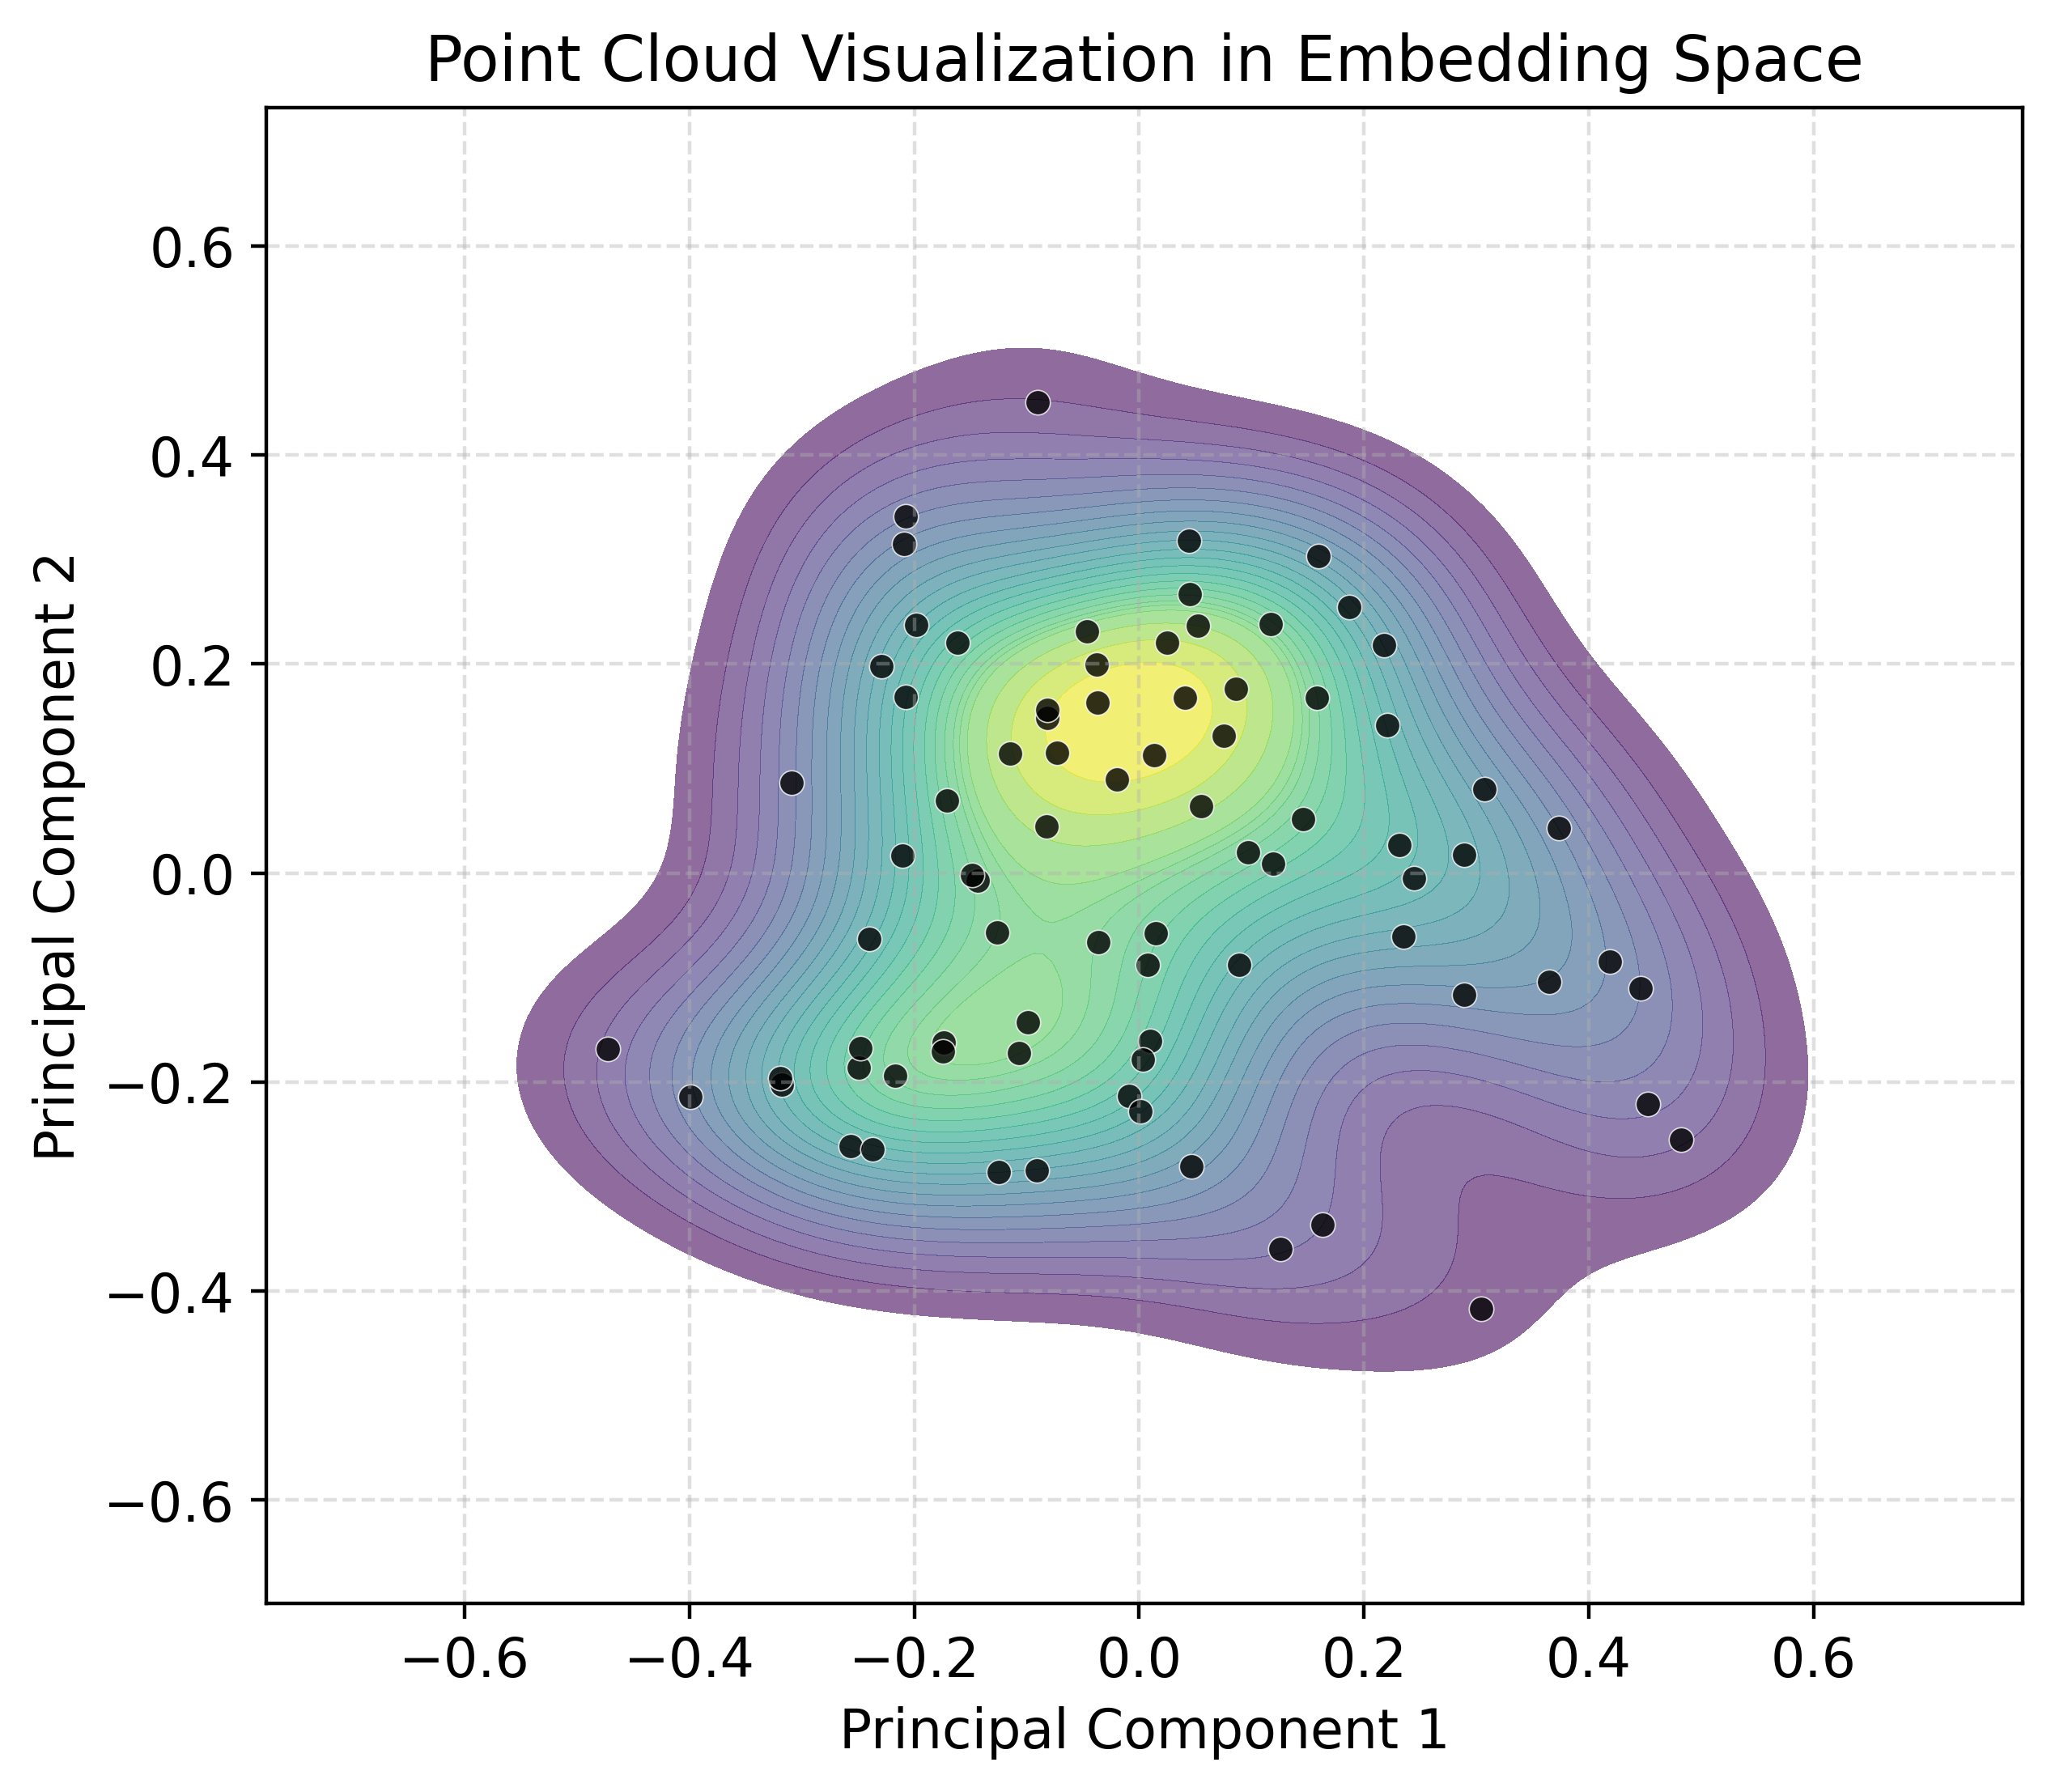
\includegraphics[width=0.75\textwidth]{point_cloud_general.png}
\caption{Point Cloud Visualization of 24 Nearest Neighbours (PCA Projection)}
\label{fig:pointcloud}
\end{figure}

As shown in \textbf{Figure~\ref{fig:pointcloud}}, the local neighbourhood of the input is
projected onto two principal components. Each point represents one of the 24 nearest neighbours,
colored by its true emotion class. A mixed-color, scattered distribution indicates that the input
sits near the boundary of multiple emotion clusters, which correlates with higher topological
complexity.

\textbf{Persistence Diagram:} This shows all H0 and H1 features plotted as
points with their birth time on the x-axis and death time on the y-axis. Points far from the
diagonal correspond to long-lived topological features, which indicate genuine structure. H1
points (loops) that are long-lived indicate that the neighbourhood has genuine topological
complexity.

\begin{figure}[H]
\centering

\includegraphics[width=0.75\textwidth]{persistence_diagram.png}
\caption{Persistence Diagram Showing H0 and H1 Topological Features}
\label{fig:persdiag}
\end{figure}

As shown in \textbf{Figure~\ref{fig:persdiag}}, each point in the persistence diagram
represents a topological feature. H0 features (connected components) appear as one group, while
H1 features (loops) appear as another. Features far from the diagonal have longer lifespans,
indicating genuine topological structure rather than noise. The number of H1 points directly
corresponds to the loop count used in the ambiguity detection rules.

\textbf{Persistence Landscape Plot:} This is the smoothed, vectorized summary of
the persistence diagram. It shows the envelope of all the persistence intervals, summarized into
a set of curves.

\begin{figure}[H]
\centering
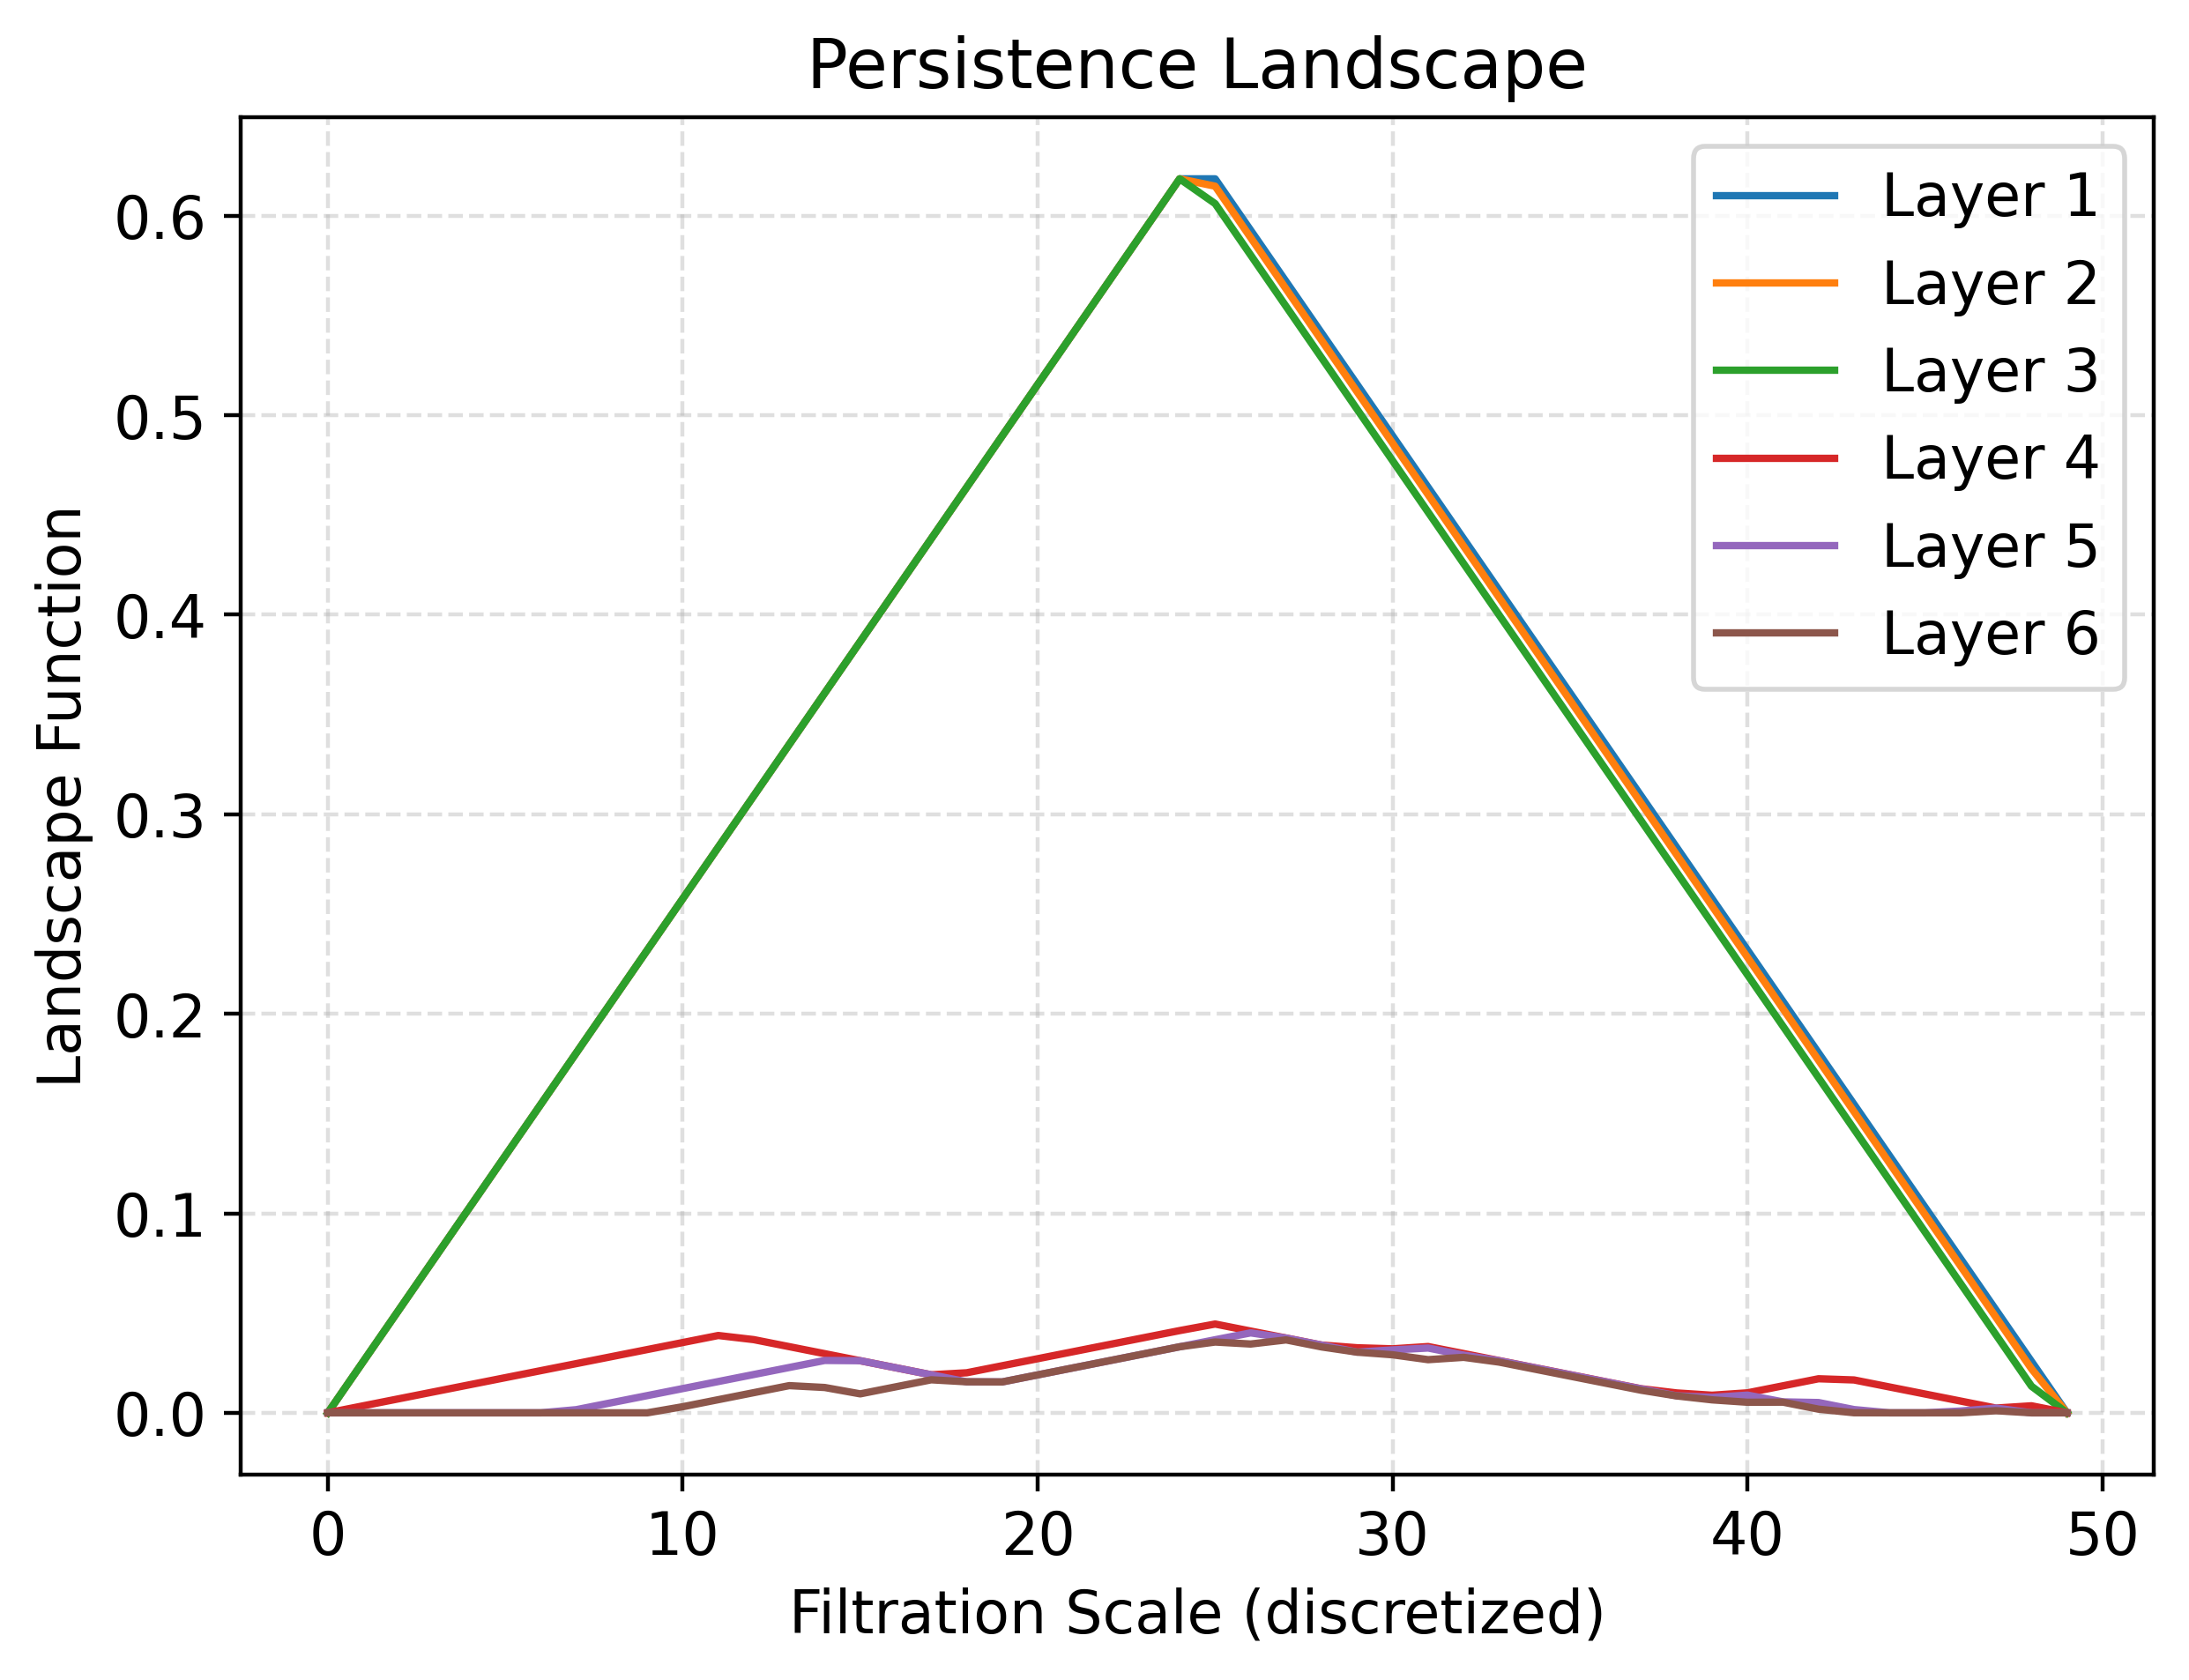
\includegraphics[width=0.75\textwidth]{persistence_landscape.png}
\caption{Persistence Landscape Representation}
\label{fig:landscape}
\end{figure}

As shown in \textbf{Figure~\ref{fig:landscape}}, the persistence landscape converts the
persistence diagram into a functional representation suitable for machine learning. The peaks
in the landscape correspond to the most prominent topological features. This vectorized
representation is concatenated with the embedding and TF-IDF features to form the final
3798-dimensional feature vector used by the classifier.

These visualizations were used during development to understand why certain inputs were being
flagged as Ambiguous and to calibrate the loop count thresholds.

\section{Model Storage}

After training, all model components are saved to a single \texttt{final\_model.joblib} file.
The file contains:

\begin{itemize}
    \item \texttt{models}: The list of three trained XGBoost classifiers.
    \item \texttt{tfidf}: The fitted TF-IDF vectorizer.
    \item \texttt{nbrs}: The fitted nearest-neighbour index.
    \item \texttt{X\_dense\_train}: The full array of training embeddings. This is needed at
    inference time to find neighbours.
    \item \texttt{VR}: The configured Vietoris-Rips persistence object.
    \item \texttt{PL}: The configured Persistence Landscape object.
\end{itemize}

The SentenceTransformer model is saved separately using its own save method, since it is a
large model that requires its own directory structure. At inference time, both are loaded at
startup.

This design means that once training is done, inference never requires internet access,
retraining, or the original dataset.
